\documentclass[UTF8]{article}
\usepackage{ctex}
\usepackage{geometry}
\usepackage{float}
\usepackage{graphicx}
\usepackage{listings}
\usepackage{subfigure}
\usepackage{amsmath}
\geometry{a4paper,scale=0.8}
\title{压力表校验及压力变送器标定实验}
\author{能动A71 宋德培 2174110112}

\renewcommand{\thesection}{\Roman{section}}
\renewcommand{\thesubsection}{\arabic{section} .\arabic{subsection}}
\usepackage{xcolor}
\lstset{
	numbers=left, 
	numberstyle= \tiny, 
	keywordstyle= \color{ blue!70},
	commentstyle= \color{red!50!green!50!blue!50}, 
	frame=shadowbox, % 阴影效果
	rulesepcolor= \color{ red!20!green!20!blue!20} ,
	escapeinside=``, % 英文分号中可写入中文
	xleftmargin=2em,xrightmargin=2em, aboveskip=1em,
	framexleftmargin=2em
} 
\begin{document}
	\maketitle
	\section{实验用仪器}
	\begin{enumerate}
	\item	活塞式压力计:用于压力表校验和压力变送器标定的专用设备。型号为YS-250,精度等级为0.05。
	\item 	标准砝码:YS-60型:0.1 MPa(4块),0.5 MPa(7块);YS-250型:2.5MPa(4块);0.5 MPa(3块)。
	\item 	被校压力表:型号YB-150;规格 0-16MPa,;精度等级1.5级。
	\item 	电容式压力变送器:压力范围 0~6 MPa,精度0.5 \%FS;压阻式压力变送器:压力范围 0~15 MPa,精度0.5\%FS,为4~20 mA电流输出型。
	\item 	Fluke 8808A数字多用表,直流电源。
	\end{enumerate}
	
	
	\section{实验原理}
	\subsection{\textit{压力表的校验}}
	压力表在使用过程中需要定期校验,以判断其准确度是否合格,
	本实验所用压力表精度等级1.5,量程15 Mpa,因此测量压力时准确度为$\pm0.225$ Mpa。 
	
	在校验时,将压力表安装在活塞式压力计上,由活塞式压力计提供在其量程内的不同的标准压力值,若在每个标准压力值下,压力表的测量误差均不超过其精度等级所允许的偏差,则该压力表合格,可以继续使用;若在任一标准压力值下,压力表的测量误差超过了其精度等级所允许的偏差,则该压力表不合格,此时需要更换压力表。
	\subsection{\textit{变送器的标定}}
	本实验使用电流型变送器,其电流输出值与压力值成线性关系,压力变送器在使用一段时间后,其输出电信号可能会发生漂移,因此,压力变送器也需要定期进行标定,以得到新的准确的压力-电信号的线性关系,或改变压力变送器变送电路的参数,将变送器的输出值重新调整为标准输出值。
	
	压力变送器标定时,将压力变送器安装在活塞式压力计上。以电流型变送器为例,由活塞式压力计提供在其量程内的不同的标准压力值,从而得到一系列电流与压力的对应关系值,根据最小二乘拟合得到电流与压力的线性关系式:
	\[
	p = a+bI
	\]
	由于本实验使用绝压型压力变送器,式中的$p$为绝对压力。
	\section{实验操作要点}
	\begin{itemize}
		\item 在实验前打开阀门$V_1$,逆时针转动手轮使泵的气缸内充满液压油
		\item 顺时针旋转手轮时一定要缓慢,否则由于压力迅速上升会将砝码座弹出
		\item 加载砝码或卸载后,转动手轮使砝码座底盘底面升起至略超过指示板上缘2~3毫米处。双手顺时针转动砝码,使底盘及砝码以不小于30转/分的初角速度旋转,以克服摩擦力的影响
		\item 首先测量上行程,然后依次卸载砝码测量下行程
		\item 一定要先降低压力计内的压力,再卸载砝码
	\end{itemize}
	\section{实验数据记录与处理}
	\subsection{\textit{原始数据记录}}
	\begin{figure}[H]
		\centering
		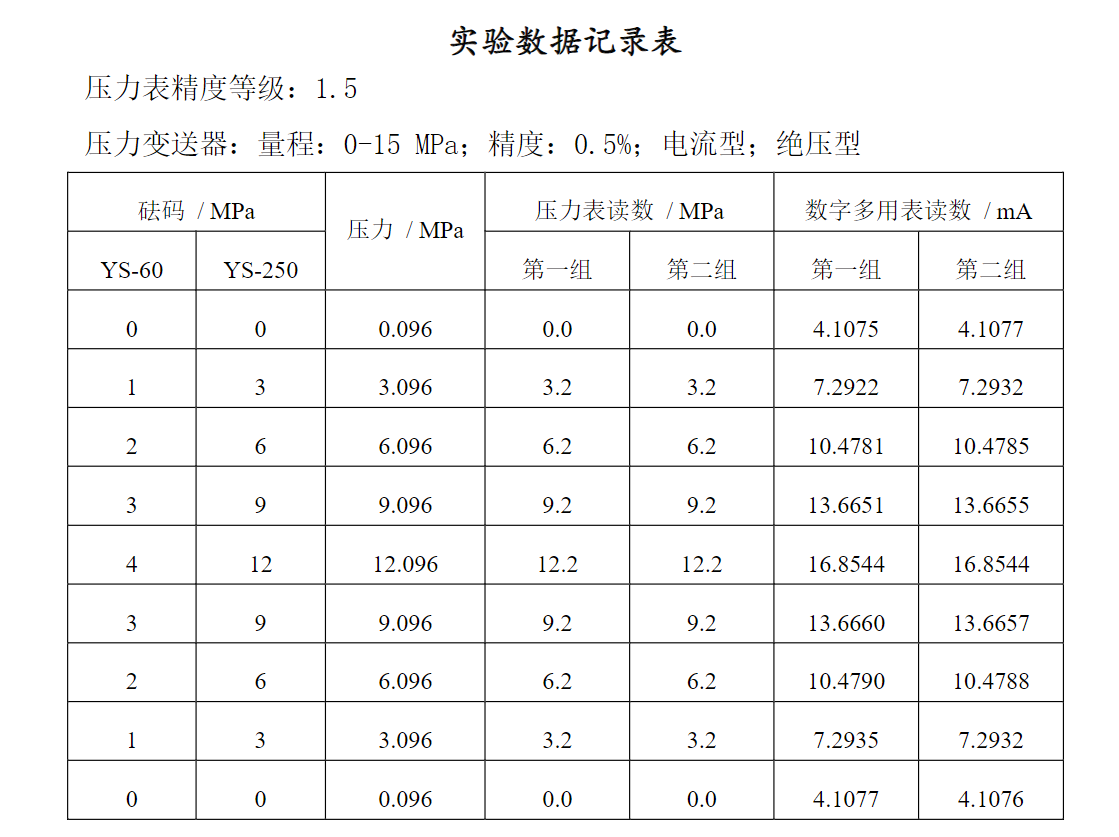
\includegraphics[width=\linewidth]{origin.png}
		\label{fig:origin}
	\end{figure}
	
	\section{作业及思考题}
	\subsection{\textit{压力表}}
	\subsubsection{上下行程曲线}
	\begin{figure}[H]
		\centering
		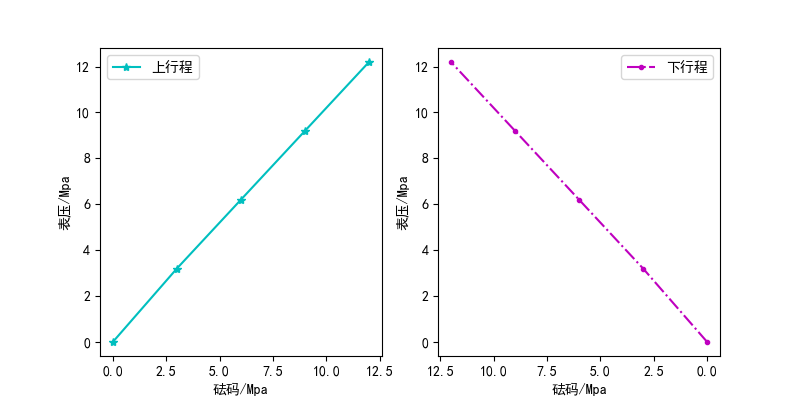
\includegraphics[width=0.7\linewidth]{Figure_1}
		\caption{压力表上下行程曲线}
		\label{fig:figure1}
	\end{figure}
	\subsubsection{校验精度}
	
	本实验所用压力表精度等级1.5,量程16 Mpa,因此测量压力时准确度为$\pm0.24$ Mpa。 而校验中最大误差为0.2Mpa,因此校验合格。
	\subsection{\textit{压力变送器}}
	
	\subsubsection{最小二乘拟合}
	
	对于更为一般的最小二乘拟合(多变量),可以将问题转换为求使得下式取得最小值的矩阵$w$
	\[
	min||\mathbf{B} - \mathbf{A}w||^2 = min\{(\mathbf{B} - \mathbf{A}w)^{T}(\mathbf{B} - \mathbf{A}w)\}
	\]
	对上式求导并令导数为零,略去其中的数学推导,可得
	\[
	w = (\mathbf{A^TA})^{-1}\mathbf{A^TB}
	\]
	在本问题中,$B$为绝对压力值组成的一维列向量,$\mathbf{A}$为输出电流及1构成的$5\times 2$的矩阵,通过编程求解,
	\begin{lstlisting}[language = python]
avg = (a1+a2+b1[::-1]+b2[::-1])/4 #average Amptitute
x = np.arange(0.096,12.097,3)
B = avg.T
A = np.array([[0.096, 3.096, 6.096, 9.096, 12.096], [1,1,1,1,1]]).T
c = A.T.dot(A)
cc = np.linalg.inv(c)
print(cc.dot(A.T.dot(B)))
	\end{lstlisting}
	得到如下的拟合直线方程
	\[
	p = 0.9414I - 3.7701
	\]
	标准关系曲线($4 \sim 20$mA)方程为
	\[
	p = 0.9375I - 3.75
	\]
	画出压力特性曲线
	\begin{figure}[H]
		\centering
		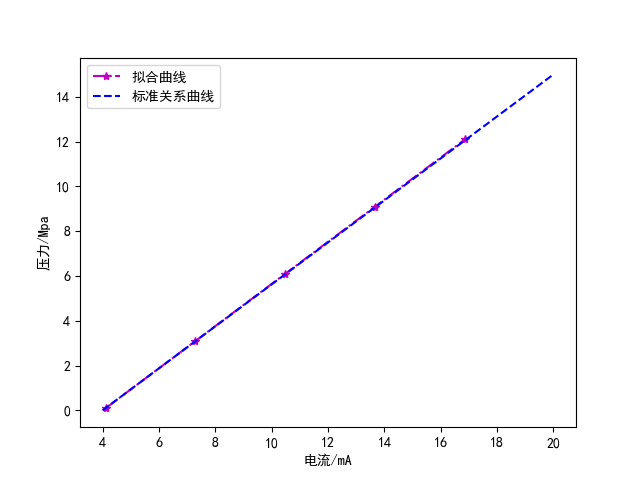
\includegraphics[width=0.7\linewidth]{fig}
		\caption{压力变送器电流-压力标准线性关系偏离图}
		\label{fig:fig}
	\end{figure}
	
	\subsubsection{实验作图}

	\begin{figure*}[htbp]
		\centering
		
		\subfigure[上下行程及拟合曲线]{
			\begin{minipage}[t]{0.5\linewidth}
				\centering
				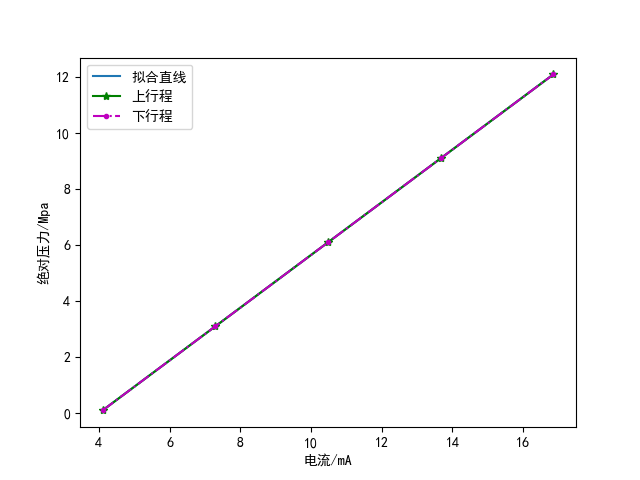
\includegraphics[width=3in]{Figure_3}\\
			\end{minipage}%
		}%
		\subfigure[压力偏差曲线]{
			\begin{minipage}[t]{0.5\linewidth}
				\centering
				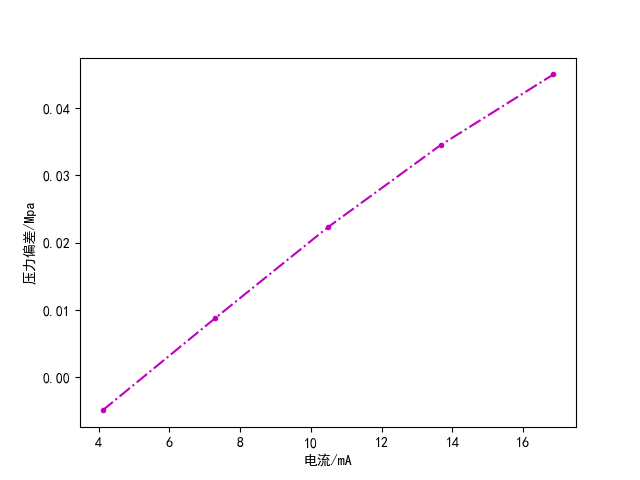
\includegraphics[width=3in]{piancha}\\
			\end{minipage}%
		}%
		
		
		\centering
		\caption{压力变送器特性曲线}
		\vspace{-0.2cm}
		\label{fig:compare_fig}
	\end{figure*}

偏差分析:从图中可以看出,压力变送器的实际特性曲线与其设计曲线并不重合,并且偏离程度随着压力的增大而增大,因此需要进行校准,重新拟合出压力-电流特性曲线,以便以后的使用。

	\subsubsection{技术指标计算}
	以压力为自变量,变送器输出电流为因变量,计算其技术指标。
	
	非线性度误差
	\begin{equation}
	\begin{split}
	\delta_{L} &= \frac{|\Delta_{max}|}{Y_{max}}\times 100\% \\
	&= 0.02045\%
	\end{split}
	\end{equation}
	
	迟滞误差
	\begin{equation}
		\begin{split}
		\delta_{H} &=\frac{|\Delta H_{m}|}{Y_{F\cdot S}} \\&=  0.003857\% 
		\end{split}
	\end{equation}
	
	重复性误差
	\begin{equation}
	\begin{split}
		\delta_{R} &=\frac{\Delta R}{Y_{F\cdot S}} \\&= 0.005933\%
	\end{split}
	\end{equation}
\end{document}